%---------------------------------------------------------------------------------------
% Propuesta de solución
%
%---------------------------------------------------------------------------------------
\DocumentMetadata{lang=es-MX}
\documentclass[stu,12pt,floatsintext,draftfirst,spanish]{report}

%-----------------------------------------PAQUETES--------------------------------------
\usepackage[spanish,mexico]{babel}
\usepackage[utf8]{inputenc}
\usepackage{times}
\usepackage{physics,amsmath,amssymb,siunitx,codehigh,cancel,float}
\usepackage{hyperref}
\usepackage{csquotes,ragged2e}
\usepackage{tabularray}
\UseTblrLibrary{booktabs}
\usepackage[x11names]{xcolor}
\usepackage{graphicx}
\usepackage[style=apa,sortcites=true,sorting=nyt,backend=biber]{biblatex}
%\addbibresource{referencias.bib}

\DeclareLanguageMapping{spanish}{spanish-apa}

%-------------------------------ESPECIFICACIONES DEL PDF--------------------------------
\hypersetup{
colorlinks=false,
pdfhighlight=/O,
pdfauthor={Jocelyn Janet Parés Ramos},
pdftitle={Propuesta de},
pdfsubject={ASUNTO DEL PDF},
pdfkeywords={PALABRAS CLAVE},
pdfproducer={LaTeX con hyperref},
pdfcreator={pdfLaTeX},
pdfstartview={Fit},
pdfpagemode={UseOutlines},
pdfnewwindow=true,
pdfpagetransition= R,
pdflang=es-MX,
}

%PORTADA--------------------------------------------------------------------------------
\title{Propuesta de solución}
\author{Jocelyn Janet Parés Ramos & 
        Juan Pablo de la Vega Lozano &
        Carlos Alberto Torre Sánchez &
        Ana Camila Murillo Fernández &
        Gael García Zúñiga}
\date{11 de abril, 2025}



%-----------------------------------------DOCUMENTO-----------------------------------------
\begin{document}
\maketitle 
 
Nuestra estrategia para resolver el problema es el modelar el sistema de John Deere con el modelo HX10 con 2 cuchillas. Primero, se debe de hacer un análisis de la situación actual del sistema, para después hacer un análisis de los parámetros que se tienen que considerar para el modelo. Las cuchillas funcionan de la siguiente manera:
\begin{figure}[htbp]
    \centering
    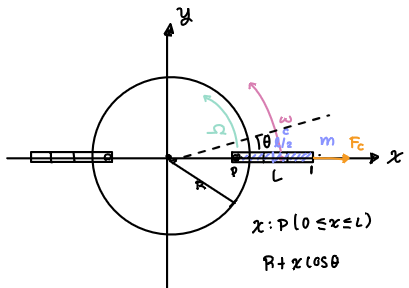
\includegraphics[width=0.5\textwidth]{diagrama.png}
    \caption{Diagrama de nuestro modelo.}
    \label{<label>}
\end{figure}
	
	
	Se tiene un disco giratorio de radio $R$ que lleva dos palas de longitud $L$, cada una unida mediante un pivote a una distancia $r < R$ del centro. Se tienen 3 ángulos, los que forman las palas respecto al radio ($\theta_1(t)$ y $\theta_2(t)$) y la del disco, que sería $\phi$ 
	
	Las variables que tenemos son:
	
	\begin{itemize}
	\item  $\phi(t)$: ángulo de rotación del disco
	\item  $\theta_i(t)$: ángulo de la cuchilla $i$ respecto a la línea radial ($i = 1, 2$)
	\item  $R$: radio del disco
	\item  $r$: distancia desde el centro al pivote de cada cuchilla
	\item  $L$: longitud de la cuchilla
	\item  $m$: masa de cuchilla
	\item  $M$: masa del disco
	\item  $b_i$: coeficiente que modela la resistencia del césped para cada cuchilla (para después usar como densidades del pasto)
	\item  $\tau_{motor}(t)$: torque que el motor aplica al disco 
	\item  $\Omega(t)$: la velocidad de rotación del disco ($\dot{\phi}(t)$).
	\end{itemize}
	
	Se quiere obtener la siguiente ecuación (con la segunda ley de newton): $\sum \tau = I \alpha$. Primero, el lado derecho de la ecuación, que sería la suma de los momentos de inercia, del disco y las cuchillas. El momento de inercia del disco se calcula como el de un disco sólido que gira alrededor de su eje:
	\begin{equation} I_{disco} = \frac{1}{2} M R^2. \end{equation}
	
	Las cuchillas se considera una varilla delgada que gira alrededor de un pivote. Para una varilla el momento de incercia se define como:
	
	$$
	I= \int_{\frac{-L}{2}}^{\frac{L}{2}}r^{2} \frac{M}{L}dr= \frac{M}{L} \frac{r^{3}}{3} \Bigg|_{\frac{-L}{2}}^{\frac{L}{2}}=\frac{M}{3L}\bigg[ \frac{L^{3}}{8}- \frac{-L^{3}}{8}\bigg]=\frac{1}{12}ML^{2}
	$$
	
	y el diferencial de masa sería $dm=\frac{M}{L}dr$
	
	No obstante, esto sera en un marco de referencia local. Por lo que tomando el teorema del eje paralelo $I=I_{c}+Md^{2}$ se obtiene que 
	$$
	\frac{1}{12} ML^{2}+Md^{2}= \frac{1}{12}ML^{2}+M \frac{L^{2}}{4}= \frac{1}{3}ML^{2}
	$$
	
	Ahora con los torques: cuando el disco gira, también las cuchillas, que igual están sometidas a fuerzas centrífugas. Para calcular el torque que estas fuerzas sobre las cuchillas, se divide en pequeñas porciones de masa $dm$, ubicadas a una distancia $x$ desde el pivote. Cada punto de la cuchilla se mueve en un círculo y experimenta una aceleración centrífuga de magnitud $a = x \dot{\phi}^2$, que genera una fuerza sobre el elemento $dm$, osea $dF = dm \cdot x \dot{\phi}^2$. Como esta fuerza está dirigida radialmente, su proyección perpendicular al eje del pivote es $dF \sin\theta$. El torque asociado es entonces:
	\begin{equation} d\tau = x \cdot dF \cdot \sin\theta\end{equation}
	
	La masa de cada segmento es $dm = \frac{m}{L} dx$. Este segmento se aleja del eje de rotación del disco a una distancia $r + x\cos\theta$, ya que la cuchilla forma un ángulo $\theta$ con la tangente del disco. Entonces su aceleración centrífuga es $(r + x\cos\theta)\dot\phi^2$, dirigida hacia afuera, que genera una fuerza
	\begin{equation}
	dF = dm \cdot a = \frac{m}{L}(r + x\cos\theta)\dot\phi^2 dx.
	\end{equation}
	
	Asimismo, como el segmento está a una distancia $x$ del pivote y la fuerza está dirigida radialmente, el componente que produce torque es la perpendicular a la cuchilla. Entonces el torque es:
	\begin{equation}
	d\tau = x\sin\theta \cdot dF = x\sin\theta \cdot \frac{m}{L}(r + x\cos\theta)\dot\phi^2 dx.
	\end{equation}
	
	Integrando desde $0$ hasta $L$:
	\begin{equation}
		\begin{aligned}
	\tau &= \int_0^L x\sin\theta \cdot \frac{m}{L}(r + x\cos\theta)\dot\phi^2 dx\\
	&= \frac{m\dot\phi^2\sin\theta}{L} \int_0^L (rx + x^2\cos\theta)\,dx
	\end{aligned}
	\end{equation}
	
	Dos integrales:
	\begin{equation}
	\int_0^L rx \,dx = r \int_0^L x \,dx = r \cdot \left[ \frac{x^2}{2} \right]_0^L = \frac{rL^2}{2},
	\end{equation}
	\begin{equation}
	\int_0^L x^2\cos\theta\,dx = \cos\theta \int_0^L x^2 \,dx = \cos\theta \cdot \left[ \frac{x^3}{3} \right]_0^L = \cos\theta \cdot \frac{L^3}{3}.
	\end{equation}
	Sustituyendo:
	\begin{equation}
	\tau = \frac{m\dot\phi^2\sin\theta}{L} \left( \frac{rL^2}{2} + \frac{L^3\cos\theta}{3} \right) = \frac{1}{2}m r L \dot\phi^2 \sin\theta + \frac{1}{3}m L^2 \dot\phi^2 \sin\theta \cos\theta.
	\end{equation}
	
	Este torque total sobre la cuchilla se debe únicamente a la componente de la fuerza centrífuga perpendicular a la pala, porque solo esa genera un corte efectivo; la componente paralela empuja a lo largo de la cuchilla y no induce rotación, por lo que no contribuye al torque.
	
	Ahora para el torque resistivo del césped, se supone que actúa como una fricción viscosa sobre cada segmento de la pala y el disco.
	
	La fuerza viscosa en el disco es
	\begin{equation}
	dF_{\rm disco} = -\,b_i\,rv_{\rm disco}\,dx
	= -\,b_i\dot\phi\,dx.
	\end{equation}
	El torque:  
	\begin{equation}
	d\tau_{\rm disco}
	= x\sin\theta \;\cdot\; dF_{\rm disco}
	= -\,x\sin\theta\;b_i\;r\dot\phi\,dx.
	\end{equation}
	Integrando 
	\begin{equation}
	\tau_{\rm disco}
	= -\,b_i\,r\dot\phi\,\sin\theta
	\int_0^L\,dx
	= -\,b_i\,r\dot\phi\,\sin\theta\frac{L^2}{2}
	\end{equation}
	
	 Cada segmento a distancia $x$ tiene dos velocidades: una por el giro del disco ($\dot\phi$), y otra por el giro propio de la cuchilla ($\dot\theta$). La velocidad tangencial debida al disco es $(r + x\cos\theta)\dot\phi$, y la debida a la rotación de la cuchilla es $x\dot\theta$. Multiplicamos cada una por un coeficiente de fricción $b_i$ y por el brazo de palanca $x\sin\theta$, luego integramos en $s$ de $0$ a $L$.
	 

	
	Tomando en cuenta el giro de la pala 
	\begin{equation}
	v_{\rm cuchilla} = x\,\dot\theta.
	\end{equation}
	La fuerza viscosa: 
	\begin{equation}
	dF_{\rm cuchilla} = -\,b_i\,x\,\dot\theta\,dx.
	\end{equation}
	Torque (brazo $x\sin\theta$):  
	\begin{equation}
	d\tau_{\rm cuchilla}
	= x\sin\theta\;\cdot\; dF_{\rm cuchilla}
	= -\,b_i\,x^2\,\dot\theta\,\sin\theta\,dx.
	\end{equation}
	Integral  
	\begin{equation}
	\tau_{\rm cuchilla}
	= -\,b_i\,\dot\theta\,\sin\theta
	\int_0^L x^2\,dx
	= -\,b_i\,\dot\theta\,\sin\theta
	\cdot \frac{L^3}{3}.
	\end{equation}
	

	Y si quitamos el signo negativo para después usarlo en \(\sum\tau=I\alpha\) como oposición al movimiento, tenemos que el total es
	\begin{equation}
	\tau_{pasto,i}
	= 
	\underbrace{\frac{1}{3}\,b_i\,L^3\,\dot\theta\,\sin\theta}_{\displaystyle\text{cuchilla}}
	\;+\;
	\underbrace{\frac12b_iL^2r\dot\phi\sin\theta}_{\displaystyle\text{disco}}
	\end{equation}

	
	Finalmente, aplicamos la segunda ley de Newton. En el disco, se tiene en el lado derecho la suma de todos los momentos de inercia y en el izquierdo sería el del motor y ambas cuchillas:
	\begin{equation} \boxed{\Big(\frac{1}{2} M R^2+\frac23mL^2\Big) \ddot{\phi} = \tau_{motor} - \sum_{i=1}^{2}\left( \frac{1}{2} b_i r L^2 \dot{\phi} \sin\theta_i + \frac{1}{3} b_i L^3 \dot{\theta}_i \right)} \end{equation}
	
	y para cada cuchilla, aplicamos la ley usando su momento de inercia ($\frac{1}{3} m L^2$) y las fuerzas centrífugas y resistivas:
	\begin{equation}
	\boxed{
	\begin{aligned}
		\frac{1}{3} m L^2 \ddot{\theta}_1 &= \left( \frac{1}{2} m r L \dot{\phi}^2 \sin\theta_1 + \frac{1}{3} m L^2 \dot{\phi}^2 \sin\theta_1 \cos\theta_1 \right) - \left( \frac{1}{2} b_1 r L^2 \dot{\phi} \sin\theta_1 + \frac{1}{3} b_1 L^3 \dot{\theta}_1 \right), \\
		\frac{1}{3} m L^2 \ddot{\theta}_2 &= \left( \frac{1}{2} m r L \dot{\phi}^2 \sin\theta_2 + \frac{1}{3} m L^2 \dot{\phi}^2 \sin\theta_2 \cos\theta_2 \right) - \left( \frac{1}{2} b_2 r L^2 \dot{\phi} \sin\theta_2 + \frac{1}{3} b_2 L^3 \dot{\theta}_2 \right)
	\end{aligned}}
	\end{equation}
	
\end{document}